\documentclass[letterpaper, 10 pt, conference]{ieeeconf}
\IEEEoverridecommandlockouts
\overrideIEEEmargins
\pdfminorversion=4
% Colors:
% Blue-ish: 8FC2FF
% Yellow-ish: FFE599
% Red-ish: FF9999
% Brown-ish: E5C07B
% Blue/Green-ish: 397880

\setcounter{secnumdepth}{3}
\usepackage{listings}
\usepackage{color}
\usepackage[hidelinks]{hyperref}
\let\proof\relax
\let\endproof\relax
\usepackage{amsmath}
\usepackage{amssymb}
\usepackage{amsthm}
\usepackage{subfig}
\usepackage{balance}
\usepackage{stfloats}
\usepackage{graphicx}
\usepackage{epstopdf}
\usepackage{bm}
\usepackage{booktabs}
\usepackage{array}
\usepackage{stfloats}
\usepackage{pdflscape}
\usepackage{pgfplots}
\usepackage{algorithm}
\usepackage{algorithmic}
\usepackage{setspace}
\usepackage{tikz}

\renewcommand{\algorithmicrequire}{\textbf{Input:}}
\renewcommand{\algorithmicensure}{\textbf{Output:}}
\renewcommand\thealgorithm{\Roman{algorithm}}

% Italics for theorems
\theoremstyle{plain}
\newtheorem{theorem}{Theorem}
\renewcommand\thetheorem{\Roman{theorem}}

% Normal for all the rest
\newtheorem{lemma}{Lemma}
\renewcommand\thelemma{\Roman{lemma}}
\newtheorem{corollary}{Corollary}
\renewcommand\thecorollary{\Roman{corollary}}
\theoremstyle{definition}
\newtheorem{problem}{Problem}
\renewcommand\theproblem{\Roman{problem}}
\newtheorem{definition}{Definition}
\renewcommand\thedefinition{\Roman{definition}}
\newtheorem{remark}{Remark}
\renewcommand\theremark{\Roman{remark}}
\newtheorem{proposition}{Proposition}
\renewcommand\theproposition{\Roman{proposition}}
\newtheorem{objective}{Objective}
\renewcommand\theobjective{\Roman{objective}}
\newtheorem{operation}{Operation}
\renewcommand\theoperation{\Roman{operation}}

\renewcommand{\qedsymbol}{$\blacksquare$}

\definecolor{mygray}{rgb}{0.5,0.5,0.5}
\definecolor{keyword}{rgb}{0.5,0.5,0.5}
\definecolor{greenCode}{rgb}{0, 0.6, 0}

\lstdefinelanguage{HTTP}{
  keywords={GET},
  ndkeywords={PUT},
  comment=[s]{PO}{T},
  morecomment=[s]{D}{LETE}
}

\lstdefinestyle{customc}{
  belowcaptionskip=1\baselineskip,
  language={HTTP},
  breaklines=true,
  frame=tb,
  captionpos=b,
  keywordstyle=\bfseries\color{greenCode},
  ndkeywordstyle=\bfseries\color{red},
  commentstyle=\bfseries\color{magenta},
  stringstyle=\bfseries\color{black},
  xleftmargin={0.75cm},
  showstringspaces=false,
  basicstyle=\footnotesize\ttfamily,
  numbers=left,
  numberstyle=\small\color{black},
}

\lstset{escapechar=@,style=customc}

%\ifCLASSINFOpdf
   %\usepackage[pdftex]{graphicx}
%\else
%\fi

\usepackage{flushend} % Equalize last page
\usepackage[colorinlistoftodos]{todonotes}


\begin{document}

\title{\LARGE \bf Scan-matching of panoramic 2D range scans}


\author{Alexandros Filotheou, Georgios D. Sergiadis, Antonis G. Dimitriou% <-this % stops a space
  \thanks{This work was supported by the European Union and Greek National Funds
  through the Operational Program Competitiveness, Entrepreneurship, and
  Innovation, under the call Research Create Innovate under Project T2EDK-02000.
  Corresponding author: Alexandros Filotheou, {\tt\small alefilot@auth.gr}.
  The authors are with the Department of Electrical and Computer Engineering,
  Aristotle University of Thessaloniki, 54124 Thessaloniki, Greece}
}

\maketitle
\thispagestyle{empty}
\pagestyle{empty}


%%%%%%%%%%%%%%%%%%%%%%%%%%%%%%%%%%%%%%%%%%%%%%%%%%%%%%%%%%%%%%%%%%%%%%%%%%%%%%%%
\begin{abstract}
  %A real-time method for matching 2D range scans extracted from a LIDAR sensor
%whose field of view is $2\pi$ is proposed. The method leverages properties of
%the Fourier transform which arise due to the periodicity of the range signal.
%The solution to scan-matching is given by transforming the problem into a
%scan--to--map-scan matching problem. Matching is performed in a
%correspondenceless manner. The proposed method outperforms established
%scan-matching methods in terms of pose accuracy and robustness in tests on
%public domain data and over sensor noise levels of commercially available range
%sensors. The source code is available for download.
%In recent years affordable but noisier 2D range sensors with a field of view of
%$2\pi$ have been introduced to the public. Scan-matching with these has been
%insufficiently researched, while being a challenge due to their
%increased measurement uncertainty. This paper proposes a real-time method for
%matching scans extracted from panoramic 2D LIDAR sensors. The method leverages
%properties of the Fourier transform which arise due to the periodicity of the
%range signal. Matching is performed in a correspondenceless manner. The
%proposed method outperforms established scan-matching methods in terms of pose
%accuracy and robustness in tests on public domain data, and over noise
%levels of commercially available sensors. The source code is available
%for download.
Recent years have seen the introduction of more affordable but less accurate 2D
range sensors whose field of view of $2\pi$. Scan-matching with these has been
insufficiently researched, while being a challenge due to these sensors'
increased measurement uncertainty. This paper proposes a real-time method for
matching scans extracted from panoramic 2D LIDAR sensors. The method leverages
properties of the Fourier transform which arise due to the periodicity of the
range signal.  Matching is performed in a correspondenceless manner. The
proposed method outperforms established scan-matching methods in terms of pose
accuracy and robustness in tests on public domain data, and over noise levels
of commercially available sensors. The source code is available for download.

\end{abstract}

\begin{keywords}
Scan-matching, localisation, panoramic LIDAR
\end{keywords}

%%%%%%%%%%%%%%%%%%%%%%%%%%%%%%%%%%%%%%%%%%%%%%%%%%%%%%%%%%%%%%%%%%%%%%%%%%%%%%%%
\section{Introduction}
  Consider a robot capable of motion, equipped with a Light Detection and Ranging
sensor (LIDAR), capturing a measurement $\mathcal{S}_0$ at time $t_0$ from pose
$\bm{p}_0$ in some reference frame. The robot then moves to pose $\bm{p}_1$ at
time $t_1$ at which time it captures measurement $\mathcal{S}_1$. Provided
overlap between the two scans, estimating the rigid-body transformation
$\bm{T}$ that projects the endpoints of $\mathcal{S}_1$ to those of
$\mathcal{S}_0$ with the least error is known as scan-matching. The solution to
the scan-matching problem is central to methods of Localisation
\cite{Ju2019}, Navigation
\cite{Kumar2018}, and Simultaneous
Localisation and Mapping (SLAM) \cite{Zhang2019,Pedrosa2020}, as
$\bm{T}$ is the rigid-body transformation $\bm{p}_1$$-$$\bm{p}_0$: i.e. the
solution to scan-matching provides localisation information at time $t_1$,
relative to $\bm{p}_0$. For this reason, along with the high measurement
accuracy of LIDAR sensors, scan-matching is also used as a means to improving,
providing, or substituting odometric measurements (where available; fig.
\ref{fig:laser_odometry}), as the latter are prone to unbounded and
unpredictable tire and wheel slippage \cite{Olson2009,Zhang2020}.

LIDAR sensors with a field of view of $360^\circ$, i.e. panoramic sensors, were
for years constrained to high price ranges, and most provided 3D measurements.
Therefore research on scan-matching with 2D LIDAR sensors mostly focused on
non-panoramic sensors, with scan matching methods being used without distinction
with regard to field of view. In recent years, however, price-appealing
panoramic 2D LIDAR sensors have emerged, but at the cost of increased measurement
uncertainty. The introduction of these sensors warrants targeted research
into scan-matching with the use of panoramic LIDAR sensors, due to (a) the
afforded periodicity of the range signal, and (b) the need of
addressing the high levels of measurement noise with regard to the
transformation errors of current scan-matching algorithms.

This paper introduces a real-time method specifically targeting the matching of
2D panoramic range scans. Its errors are largely invariant to angular and
locational displacement for a given level of measurement noise. The central
contributions of the paper are:

\begin{itemize}
  \item To the best of the author's knowledge, the first method explicitly
        addressing the matching of panoramic 2D range scans that operates
        without establishing correspondences between input scans
  \item The extrication from the need of a prior transformation estimate
  \item The introduction of a method that aims at reducing the orientation
        error to lower than the sensor's angle increment compared to relevant
        prior work
  \item The parameter set needed by the proposed method is intuitive, smaller
        than those of established methods, and trades accuracy for execution
        time
  \item The thorough evaluation of the proposed method against five established
        scan-matching algorithms in common use, over five benchmark datasets
        and measurement noise levels from common-use, commercially
        available sensors
\end{itemize}

\begin{figure}[]\centering
  \vspace{-1.3cm}
  % GNUPLOT: LaTeX picture with Postscript
\begingroup
  \makeatletter
  \providecommand\color[2][]{%
    \GenericError{(gnuplot) \space\space\space\@spaces}{%
      Package color not loaded in conjunction with
      terminal option `colourtext'%
    }{See the gnuplot documentation for explanation.%
    }{Either use 'blacktext' in gnuplot or load the package
      color.sty in LaTeX.}%
    \renewcommand\color[2][]{}%
  }%
  \providecommand\includegraphics[2][]{%
    \GenericError{(gnuplot) \space\space\space\@spaces}{%
      Package graphicx or graphics not loaded%
    }{See the gnuplot documentation for explanation.%
    }{The gnuplot epslatex terminal needs graphicx.sty or graphics.sty.}%
    \renewcommand\includegraphics[2][]{}%
  }%
  \providecommand\rotatebox[2]{#2}%
  \@ifundefined{ifGPcolor}{%
    \newif\ifGPcolor
    \GPcolorfalse
  }{}%
  \@ifundefined{ifGPblacktext}{%
    \newif\ifGPblacktext
    \GPblacktexttrue
  }{}%
  % define a \g@addto@macro without @ in the name:
  \let\gplgaddtomacro\g@addto@macro
  % define empty templates for all commands taking text:
  \gdef\gplbacktext{}%
  \gdef\gplfronttext{}%
  \makeatother
  \ifGPblacktext
    % no textcolor at all
    \def\colorrgb#1{}%
    \def\colorgray#1{}%
  \else
    % gray or color?
    \ifGPcolor
      \def\colorrgb#1{\color[rgb]{#1}}%
      \def\colorgray#1{\color[gray]{#1}}%
      \expandafter\def\csname LTw\endcsname{\color{white}}%
      \expandafter\def\csname LTb\endcsname{\color{black}}%
      \expandafter\def\csname LTa\endcsname{\color{black}}%
      \expandafter\def\csname LT0\endcsname{\color[rgb]{1,0,0}}%
      \expandafter\def\csname LT1\endcsname{\color[rgb]{0,1,0}}%
      \expandafter\def\csname LT2\endcsname{\color[rgb]{0,0,1}}%
      \expandafter\def\csname LT3\endcsname{\color[rgb]{1,0,1}}%
      \expandafter\def\csname LT4\endcsname{\color[rgb]{0,1,1}}%
      \expandafter\def\csname LT5\endcsname{\color[rgb]{1,1,0}}%
      \expandafter\def\csname LT6\endcsname{\color[rgb]{0,0,0}}%
      \expandafter\def\csname LT7\endcsname{\color[rgb]{1,0.3,0}}%
      \expandafter\def\csname LT8\endcsname{\color[rgb]{0.5,0.5,0.5}}%
    \else
      % gray
      \def\colorrgb#1{\color{black}}%
      \def\colorgray#1{\color[gray]{#1}}%
      \expandafter\def\csname LTw\endcsname{\color{white}}%
      \expandafter\def\csname LTb\endcsname{\color{black}}%
      \expandafter\def\csname LTa\endcsname{\color{black}}%
      \expandafter\def\csname LT0\endcsname{\color{black}}%
      \expandafter\def\csname LT1\endcsname{\color{black}}%
      \expandafter\def\csname LT2\endcsname{\color{black}}%
      \expandafter\def\csname LT3\endcsname{\color{black}}%
      \expandafter\def\csname LT4\endcsname{\color{black}}%
      \expandafter\def\csname LT5\endcsname{\color{black}}%
      \expandafter\def\csname LT6\endcsname{\color{black}}%
      \expandafter\def\csname LT7\endcsname{\color{black}}%
      \expandafter\def\csname LT8\endcsname{\color{black}}%
    \fi
  \fi
    \setlength{\unitlength}{0.0500bp}%
    \ifx\gptboxheight\undefined%
      \newlength{\gptboxheight}%
      \newlength{\gptboxwidth}%
      \newsavebox{\gptboxtext}%
    \fi%
    \setlength{\fboxrule}{0.5pt}%
    \setlength{\fboxsep}{1pt}%
\begin{picture}(5000.00,5000.00)%
    \gplgaddtomacro\gplbacktext{%
      \colorrgb{0.15,0.15,0.15}%
      \put(391,1564){\makebox(0,0)[r]{\strut{}$6.0$}}%
      \colorrgb{0.15,0.15,0.15}%
      \put(391,1988){\makebox(0,0)[r]{\strut{}$8.0$}}%
      \colorrgb{0.15,0.15,0.15}%
      \put(391,2413){\makebox(0,0)[r]{\strut{}$10.0$}}%
      \colorrgb{0.15,0.15,0.15}%
      \put(391,2837){\makebox(0,0)[r]{\strut{}$12.0$}}%
      \colorrgb{0.15,0.15,0.15}%
      \put(391,3262){\makebox(0,0)[r]{\strut{}$14.0$}}%
      \colorrgb{0.15,0.15,0.15}%
      \put(391,3687){\makebox(0,0)[r]{\strut{}$16.0$}}%
      \colorrgb{0.00,0.00,0.00}%
      \put(672,1280){\makebox(0,0){\strut{}$-2.0$}}%
      \colorrgb{0.00,0.00,0.00}%
      \put(1096,1280){\makebox(0,0){\strut{}$0.0$}}%
      \colorrgb{0.00,0.00,0.00}%
      \put(1521,1280){\makebox(0,0){\strut{}$2.0$}}%
      \colorrgb{0.00,0.00,0.00}%
      \put(1945,1280){\makebox(0,0){\strut{}$4.0$}}%
      \colorrgb{0.00,0.00,0.00}%
      \put(2370,1280){\makebox(0,0){\strut{}$6.0$}}%
    }%
    \gplgaddtomacro\gplfronttext{%
    }%
    \gplgaddtomacro\gplbacktext{%
      \colorrgb{0.00,0.00,0.00}%
      \put(2822,1280){\makebox(0,0){\strut{}$-2.0$}}%
      \colorrgb{0.00,0.00,0.00}%
      \put(3246,1280){\makebox(0,0){\strut{}$0.0$}}%
      \colorrgb{0.00,0.00,0.00}%
      \put(3671,1280){\makebox(0,0){\strut{}$2.0$}}%
      \colorrgb{0.00,0.00,0.00}%
      \put(4095,1280){\makebox(0,0){\strut{}$4.0$}}%
      \colorrgb{0.00,0.00,0.00}%
      \put(4520,1280){\makebox(0,0){\strut{}$6.0$}}%
    }%
    \gplgaddtomacro\gplfronttext{%
    }%
    \gplbacktext
    \put(0,0){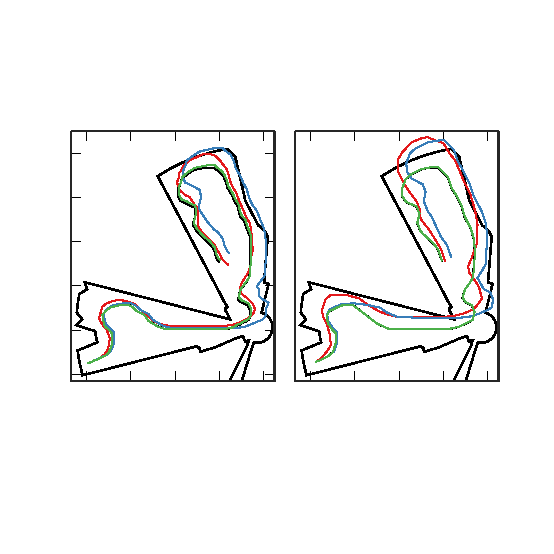
\includegraphics{./figures/odom_test_5_vs_6}}%
    \gplfronttext
  \end{picture}%
\endgroup

  \vspace{-2cm}
  \caption{\small Scan-matching as ``laser odometry": the robot moves from the
           lower left portion of the environment to the upper right, capturing
           2D range scans along its trajectory. The coloured routes show the
           estimated path of the robot derived from each method. The proposed
           method's error is invariant to angular and locational displacement}
  \label{fig:laser_odometry}
\end{figure}

The rest of the paper is structured as follows. In section
\ref{section:definitions_and_problem_formulation} necessary notions are
defined, and the problem of matching panoramic 2D range scans is formulated. A
brief review of methods matching 2D range scans is given in section
\ref{section:sota}. Section \ref{section:the_proposed_method} provides an
analysis of the proposed method. The experimental setup and are illustrated in
section \ref{section:results}. Section \ref{section:characterisation} gives
characterisations of the proposed method compared to state of the art methods.
Section \ref{section:finale} concludes this paper.


%%%%%%%%%%%%%%%%%%%%%%%%%%%%%%%%%%%%%%%%%%%%%%%%%%%%%%%%%%%%%%%%%%%%%%%%%%%%%%%%
\section{Definitions}
  \label{section:definitions}
  %%%%%%%%%%%%%%%%%%%%%%%%%%%%%%%%%%%%%%%%%%%%%%%%%%%%%%%%%%%%%%%%%%%%%%%%%%%%%%%%
\begin{definition}
  \label{def:definition_1}
  \textit{Definition of a range scan captured from a conventional 2D LIDAR
  sensor.} A conventional 2D LIDAR sensor provides a finite number of ranges,
  i.e. distances to objects within its range, on a horizontal cross-section of
  its environment, at regular angular and temporal intervals, over a defined
  angular range \cite{lidar}. We define a range scan $\mathcal{S}$, consisting
  of $N_s$ rays over an angular range $\lambda$, to be an ordered map
  $\mathcal{S} : \Theta \rightarrow \mathbb{R}_{\geq 0}$, where $\Theta =
  \{\theta_n \in [-\frac{\lambda}{2}, +\frac{\lambda}{2}) : \theta_n =
  -\frac{\lambda}{2} + \lambda \frac{n}{N_s}$, $n = 0,1,\dots, N_s$$-$$1$$\}$.
  Angles $\theta_n$ are expressed relative to the sensor's heading, in the
  sensor's frame of reference.
\end{definition}

%%%%%%%%%%%%%%%%%%%%%%%%%%%%%%%%%%%%%%%%%%%%%%%%%%%%%%%%%%%%%%%%%%%%%%%%%%%%%%%%
\begin{definition}
  A LIDAR sensor's angle increment $\gamma$ is the angular distance between two
  consecutive rays: $\gamma \triangleq \dfrac{\lambda}{N_s}$
\end{definition}

%%%%%%%%%%%%%%%%%%%%%%%%%%%%%%%%%%%%%%%%%%%%%%%%%%%%%%%%%%%%%%%%%%%%%%%%%%%%%%%%
\begin{definition}
  \label{def:definition_2}
  \textit{Scan-matching (or scan-to-scan matching) using a 2D LIDAR sensor} (adapted for use in
  two dimensions from \cite{plicp}).
  Let two range scans as defined by Definition \ref{def:definition_1},
  $\mathcal{S}_R$ and $\mathcal{S}_V$, be captured from a LIDAR
  sensor operating in the same environment at both capturing times. Let
  $\bm{p}_V(x_V,y_V,\theta_V)$ be the pose from
  which the sensor captured $\mathcal{S}_V$, expressed in some coordinate
  system (usually a past pose estimate of the sensor). The objective of
  scan-matching in two dimensions is to find the roto-translation
  $\bm{q} = (\bm{t}, \theta)$, $\bm{t} = (\Delta x, \Delta y)$ that minimises
  the distance of the endpoints of $\mathcal{S}_V$ roto-translated by
  $\bm{q}$ to their projection on $\mathcal{S}_R$. Denoting the
  endpoints of $\mathcal{S}_V$ by $\{\bm{p}_V^i\}$, in formula:
  \begin{align}
    \underset{\bm{q}}{\min} \sum\limits_i \Big\| \bm{p}_V^i \oplus \bm{q} - \prod \{ \mathcal{S}_R, \bm{p}_V^i \oplus \bm{q} \}\Big\|^2
    \label{eq:s2sm_def}
  \end{align}
  The symbol ``$\oplus$" denotes the roto-translation operator
  $\bm{p}_V^i \oplus (\bm{t}, \theta) \triangleq \bm{R}(\theta) \bm{p}^i_V + \bm{t}$,
  where $\bm{R}(\theta)$ is the 2D rotation matrix for argument angle $\theta$,
  and $\prod\{\mathcal{S}_R, \bm{p}_V^i \oplus \bm{q} \}$ denotes
  the Euclidean projector on $\mathcal{S}_R$.
\end{definition}


%%%%%%%%%%%%%%%%%%%%%%%%%%%%%%%%%%%%%%%%%%%%%%%%%%%%%%%%%%%%%%%%%%%%%%%%%%%%%%%%
\begin{remark}
  Scan-matching is employed in robotics as a means to odometry,
  primarily in non-wheeled robots where no encoders can be utilised, or as a
  useful ameliorator of the ever-drifting encoder-ed odometry: scans captured at
  consecutive time instances, inputted to a scan-matching algorithm, convey an
  estimate as to the pose of the scan sensor at the second capture time
  relative to that captured first. Scan-matching is being successfully employed
  in the tasks of simultaneous localisation and mapping
  \cite{am_odom_1}-\cite{am_odom_3}, local map construction
  \cite{am_odom_4}-\cite{am_odom_6}, and in people-tracking systems
  \cite{am_odom_7}.
\end{remark}

%%%%%%%%%%%%%%%%%%%%%%%%%%%%%%%%%%%%%%%%%%%%%%%%%%%%%%%%%%%%%%%%%%%%%%%%%%%%%%%%
\begin{definition}
  \label{def:definition_3}
  \textit{Definition of a map-scan.}
  A map-scan is a virtual scan that encapsulates the same pieces of information
  as a scan derived from a physical sensor. Only their underlying operating
  principle is different due to the fact the map-scan refers to distances to
  obstacles within the map ---hence its virtuality. A map-scan is captured from
  a virtual sensor and derived by means of locating intersections of rays
  emanating from the estimate of the sensor's pose and boundaries demarcating
  obstacles in the map.
\end{definition}


%%%%%%%%%%%%%%%%%%%%%%%%%%%%%%%%%%%%%%%%%%%%%%%%%%%%%%%%%%%%%%%%%%%%%%%%%%%%%%%%
\section{Problem Formulation}
  \label{section:the_problem}
  \begin{problem}
  \label{prob:the_problem}
  Let a mobile robot, capable of motion in the $x-y$ plane, be equipped with a
  coplanarly mounted range scan sensor emitting $N_s$ rays. Let
  also the following be available or standing:
  \begin{itemize}
    \item The angular range of the range sensor is $360^\circ$
    \item A 2D range scan $\mathcal{S}_0$, captured at time $t_0$
    \item A 2D range scan $\mathcal{S}_1$, captured at $t_1 > t_0$
  \end{itemize}
\end{problem}
Then the objective is estimating the 3D rigid-body transformation
$\bm{T} = (\Delta x, \Delta y, \Delta \theta)$ which, when applied to the
endpoints of $\mathcal{S}_1$, aligns them to those of $\mathcal{S}_0$ with the
least error. Equivalently, roto-translation $\bm{T}$ corresponds to the
relative motion of the sensor from the pose where it captured $\mathcal{S}_0$
to the pose from which it captured $\mathcal{S}_1$.


%%%%%%%%%%%%%%%%%%%%%%%%%%%%%%%%%%%%%%%%%%%%%%%%%%%%%%%%%%%%%%%%%%%%%%%%%%%%%%%%
\section{Prior Work}
  \label{section:sota}
  Scan-matching with the use of a 2D LIDAR sensor began with IDC \cite{LuMilios},
an algorithm incorporating elements of the Iterative Closest Point (ICP)
algorithm \cite{ICP}. The latter and its variants, e.g.
\cite{weighted}-\cite{plicp}, have become the de facto scan-matching algorithms
in 2D and 3D settings, and research using ICP is still ongoing
\cite{ICP_var_1}-\cite{Marchel}. In particular, PL-ICP \cite{plicp} has been
widely adopted due to its increased accuracy among ICP variants, and the
availability of its source code. ICP and its variants, however, exhibit varying
performance \cite{icp_comp_trade}, limited by the noise level in the input
scans, the choice of prior, and the configuration of the parameters
governing their response. For these reasons, as well as for reasons of
robustness, the method of establishing correspondences shifted from
point-to-point or point-to-line to feature-to-feature. Commonly appearing
features for recognition are line segments \cite{CLS}-\cite{Wen}, corners
\cite{wang}, SIFT features \cite{Jiayuan}, or features extracted through the
use of deep learning techniques \cite{Jiaxin}\cite{li}. In parallel, and for
reasons of independency from chance features or tailoring methods to specific
circumstances, research sprung around methods that extract or exploit
mathematical properties from range scans, or that view the problem of
scan-matching as an optimisation problem. Examples include correlation-based
methods \cite{olson},\cite{olson_2015}-\cite{Konecny}, feature distribution
matching \cite{HSM}, matching by cost function minimisation \cite{PB_PSM}, and
probabilistic methods \cite{pIC}\cite{gpm}. Among the latter, the Normal
Distributions Transform (NDT) \cite{ndt1} has gained popularity due to its
explicit modeling of measurement and pose uncertainties and its extensibility
to three dimensions \cite{ndt2}-\cite{ndt7}.

The method introduced in this paper is most akin to those of \cite{Heng} and
\cite{Jiang}. They use POMF \cite{fmt2d} in both rotation and translation
components; the latter in two dimensions and the former in one dimension. In
the latter, the requirements for a real-time solution and adequate accuracy
could not be fulfilled simultaneously. Therefore a rough output was used as an
input prior to ICP in order to overcome the problem. In the former, the
orientation error is limited by the range sensor's immutable angle increment,
but no mitigation technique is employed. Secondly, the translation component
operates in discrete space, thereby being susceptible to discretisation errors
and larger execution times as resolution increases. By contrast, the method
introduced in this paper addresses all the above issues by (a) fulfilling the
real-timeness constraint, (b) aiming at extricating the orientation error from
the sensor's angle increment, and (c) employing a continuous-space translation
method. A detailed review of scan-matching methods may be found in
\cite{pose_selection}.


%%%%%%%%%%%%%%%%%%%%%%%%%%%%%%%%%%%%%%%%%%%%%%%%%%%%%%%%%%%%%%%%%%%%%%%%%%%%%%%%
\section{Approach}
  \label{section:the_proposed_method}
  The problem is iteratively decomposed into two disjunctive sub-problems. The
first is estimating the relative angle between $\mathcal{S}_1$ and
$\mathcal{S}_0$ under the assumption that both are captured from the same
location. The second is estimating the relative displacement of $\mathcal{S}_1$
with respect to $\mathcal{S}_0$ under the assumption that both are captured
from poses of the same orientation. Solving the first sub-problem is followed
by the solution to the second sub-problem. This process is iterated until
termination conditions are met.

The orientation and location correction submethods are presented in subsections
\ref{subsec:method_orientation_correction} and
\ref{subsec:method_location_correction}. Subsection
\ref{subsec:method_pose_correction} presents the method of how these two
are woven together into the system that solves Problem \ref{prob:the_problem}
that is proposed in this work.

\subsection{Orientation Correction}
  \label{subsec:method_orientation_correction}
  Let the assumptions of Problem \ref{prob:the_problem} be standing. Assume that
the two scans were captured from the same location but from different
orientations. Denoting with $\mathcal{F}\{\mathcal{S}\}$ the Discrete Fourier
Transform of signal $\mathcal{S}$, with $\mathcal{F}^{-1}\{\mathcal{S}\}$
its inverse, and with $\bm{c}^\ast$ the conjugate of complex $\bm{c}$, calculate
$Q_{\mathcal{S}_0, \mathcal{S}_1}$:
\begin{align}
  Q_{\mathcal{S}_0, \mathcal{S}_1} \triangleq \dfrac{\mathcal{F}\{\mathcal{S}_0\}^{\ast} \cdot \mathcal{F}\{\mathcal{S}_1\}}{|\mathcal{F}\{\mathcal{S}_0\}| \cdot |\mathcal{F}\{\mathcal{S}_1\}|}
\end{align}
on the basis that if space is sampled sufficiently densely, for
$k,\xi \in [0, N_s-1]$, $k,\xi \in \mathbb{Z}$:
\begin{align}
  \mathcal{S}_0[k] &\simeq \mathcal{S}_1[(k - \xi) \mod N_s] \Leftrightarrow \nonumber \\
  \mathcal{F}\{\mathcal{S}_0\}(u) &\simeq e^{-j 2\pi \xi u / N_s} \cdot \mathcal{F}\{\mathcal{S}_1\}(u) \nonumber
\end{align}
and therefore since $2\pi \dfrac{\xi}{N_s} = \xi \dfrac{2\pi}{N_s} = \xi \gamma$

\begin{align}
  Q_{\mathcal{S}_0, \mathcal{S}_1}(u) &= \dfrac{\mathcal{F}\{\mathcal{S}_0\}^{\ast} \cdot \mathcal{F}\{\mathcal{S}_1\}}{|\mathcal{F}\{\mathcal{S}_0\}| \cdot |\mathcal{F}\{\mathcal{S}_1\}|}  \nonumber \\
  &\simeq \dfrac{e^{-j \xi \gamma  u} \cdot \mathcal{F}\{\mathcal{S}_1\}^\ast \cdot \mathcal{F}\{\mathcal{S}_1\}}{|e^{-j \xi \gamma u} \cdot \mathcal{F}\{\mathcal{S}_1\}^\ast | \cdot | \mathcal{F}\{\mathcal{S}_1\}|} \nonumber \\
  &= e^{-j \xi \gamma u} \cdot \dfrac{\mathcal{F}\{\mathcal{S}_1\}^\ast \cdot \mathcal{F}\{\mathcal{S}_1\}}{|\mathcal{F}\{\mathcal{S}_1\} | \cdot | \mathcal{F}\{\mathcal{S}_1\}|} \nonumber \\
  &= e^{-j \xi \gamma u}
  \label{eq:Q0}
\end{align}
The inverse of $Q_{\mathcal{S}_0, \mathcal{S}_1}$ is a Kronecker
$\delta$-function
$q_{\mathcal{S}_0, \mathcal{S}_1} = \mathcal{F}^{-1}\{Q_{\mathcal{S}_0, \mathcal{S}_1}\}$
centered at $\xi$:
\begin{align}
  \xi = \operatorname*{arg\,max}\limits_u \ q_{\mathcal{S}_0, \mathcal{S}_1}(u)
\end{align}
If the difference in orientation between the two scans is $\Delta\theta$, then
$\Delta\theta = \xi\gamma + \delta\theta$, where
$\mod(|\delta\theta|, \gamma) = \lambda \in [0,\frac{\gamma}{2}]$. Therefore for
a given number of emitted rays $N_s$ there remains an unresolved orientation
error $|\delta\theta| \leq \gamma/2$. The contribution of this error to the
scan-matching error is two-fold, as its existence is also propagated to the
location estimation method. In the following, a method for further reduction of
the orientation error is presented.

Let $\mathcal{S}_0$ be projected onto the 2D plane around an arbitrary but
fixed pose $\bm{p}_0(x_0, y_0, \theta_0)$, producing point-set $\bm{M}_R$, which
will hereafter be referred to as the map. Then compute $2^\nu$ map-scans (def.
\ref{def:definition_3}) $\mathcal{S}_0^k$, $k = 0,\dots,2^\nu-1$, starting from
orientation $\theta_0$, at $\gamma / 2^\nu$ angular increments. Then the
orientation estimation process is carried out once between $\mathcal{S}_1$ and
map scan $\mathcal{S}_0^k$ taken from orientation $\theta_0^k = \theta_0 +
k \cdot \gamma / 2^\nu$, for a total of $2^\nu$ times. An alignment metric
between the $k$-th map scan $\mathcal{S}_0^k$ and scan $\mathcal{S}_1$ is
computed according to
\begin{align}
  \text{PD}_k = \dfrac{2 \max q_{\mathcal{S}_0^k,\mathcal{S}_1}}{\max q_{\mathcal{S}_0^k,\mathcal{S}_0^k} + \max q_{\mathcal{S}_1,\mathcal{S}_1}}
  \label{eq:pd}
\end{align}

The Percent Discrimination metric PD$_k$ $\in [0,1]$, and is proportional to
the degree of alignment between map-scan $\mathcal{S}_0^k$ and
scan $\mathcal{S}_1$, across all $2^\nu$ map-scans $\mathcal{S}_0^k$.
The above analysis is the equivalent of the 2D Fourier-Mellin Invariant
matching in one dimension \cite{fmt2d}.

Let now $K$ denote the index of the $k$-th map scan
$\mathcal{S}_0^K$ scoring the highest PD$_k$: $\text{PD}_K =
\max \{\text{PD}_k\}$, $k = 0,\dots,2^\nu-1$. Let also $\Xi$ denote the integer
multiple of angle increments $\gamma$ by which $\mathcal{S}_V^K$
should be rotated counter-clockwise in order to achieve PD$_K$:
$\Xi = \arg\max\ q_{\mathcal{S}_0^K, \mathcal{S}_1}$.  Then the sensor's
orientation difference becomes
$\Delta\theta = \Xi\gamma + K \cdot \gamma/2^\nu + \delta\theta^\prime$.
?? Consider CAER here ??

If map-scans $\mathcal{S}_V^k$ were computed by raycasting the map of the
environment instead of $\bm{M}_R$ then the residual and unresolved orientation
error $|\delta\theta^\prime| \in [0,\gamma / 2^{1+\nu}]$. In this case, however,
$\bm{M}_R$ is an approximation of the environment's map in the locality of
$\bm{p}_0$. Depending on the magnitude of the sensor's angle increment and
the arbitrariness of the environment, this approximation may be viewed as
induced local perturbations in the map of the environment. This holds true
in the general case as well, where $\mathcal{S}_0$ and $\mathcal{S}_1$ are
captured from different locations. Therefore the guarantee of
$|\delta\theta^\prime| \leq \gamma / 2^{1+\nu}$ may not always hold for all
combinations of environments and sensor angle increments.


\subsection{Location Correction}
  \label{subsec:method_location_correction}
  Let the assumptions of Problem \ref{prob:the_problem} hold. Assume now
that $\mathcal{S}_0$ and $\mathcal{S}_1$ were captured from different
positions in the same environment but with the same orientation
relative to a fixed reference frame. Let $\mathcal{S}_0$ be projected onto
the $x-y$ plane around pose $\bm{s}(0,0,0)$,
producing point-set $\bm{M}_L$. Assuming that $\mathcal{S}_1$ was captured in a
neighbourhood of $\mathcal{S}_0$, then $\bm{M}_L$ is a perturbed local map of
the environment with respect to sensor measurement $\mathcal{S}_1$. Aside from
measurement noise, this perturbation manifests due to the finiteness of the
sensor's angle increment and to the fact that different portions of the
environment are perceptible and therefore measurable from different locations
\cite{olson}. The nature of these perturbations on map-scans captured within
$\bm{M}_L$ is additive and finite. Under these assumptions the problem of
(scan-)matching scan $\mathcal{S}_1$ to scan $\mathcal{S}_0$ may be transformed
into a problem of scan--to--map-scan matching, where the aim is registering
scan $\mathcal{S}_1$ to map $\bm{M}_L$: i.e. estimating the pose $\bm{p}_1$
from where $\mathcal{S}_1$ was captured within $\bm{M}_L$. Theorem
\ref{prop:theorem_with_disturbance} guarantees that the error of the location
estimate between the poses from which the two scans were captured is bounded in
a neighbourhood of the origin, if the location component of the pose estimate
of $\bm{p}_1$ is treated according to Theorem
\ref{prop:theorem_without_disturbance}, when its initial value is set to
$\hat{\bm{p}}_1 = \bm{s}$.


\begin{theorem}
  \label{prop:theorem_without_disturbance}
  Let a panoramic 2D range scan $\mathcal{S}_R$ be captured from a physical
  range sensor from unknown pose $\bm{p} = (\bm{l},\theta)$, $\bm{l} = (x,y)$.
  Let $\bm{M}$ be the map of the world in which the scan was captured. Let a
  pose estimate $\hat{\bm{p}} = (\hat{\bm{l}}, \hat{\theta})$ reside in the
  neighbourhood of $\bm{p}$ in the map's frame of reference. Additionally, let
  $\hat{\theta} = \theta$. Assume that $\mathcal{S}_R$ is disturbance-free,
  and that the map of the environment captures the latter perfectly. Then,
  treating the estimate of the location of the sensor as a state variable
  $\hat{\bm{l}}[k] = [\hat{x}[k], \hat{y}[k]]^\top$ and updating it according
  to the difference equation
  \begin{align}
    \hat{\bm{l}}[k+1] = \hat{\bm{l}}[k] + \bm{u}[k]
    \label{eq:difference_equation_without_disturbance}
  \end{align}
  where $\hat{\bm{l}}[0] = \hat{\bm{l}} = [\hat{x}, \hat{y}]^{\top}$,
  i.e. the supplied initial location estimate, where
  \begin{align}
    \bm{u}[k] = \dfrac{1}{N_s}
    \begin{bmatrix}
      \cos\hat{\theta} & \sin\hat{\theta} \\
      \sin\hat{\theta} & - \cos\hat{\theta}
    \end{bmatrix}
    \begin{bmatrix}
      X_{1,r}\big(\mathcal{S}_R, \mathcal{S}_V|_{\bm{\hat{p}}[k]}\big) \vspace{0.2cm} \\
      X_{1,i}\big(\mathcal{S}_R, \mathcal{S}_V|_{\bm{\hat{p}}[k]}\big)
    \end{bmatrix}
    \label{eq:control_vector_without_disturbance}
  \end{align}
  is the two-dimensional vector hereafter referred to as the
  \textit{control vector}, with
  $X_{1,r}(\cdot)$ and $X_{1,i}(\cdot)$ being, respectively, the real and
  imaginary parts of the complex quantity $X_1$:
  \begin{align}
    X_1\big(\mathcal{S}_R, \mathcal{S}_V|_{\bm{\hat{p}}[k]}\big) =
      &X_{1,r}\big(\mathcal{S}_R, \mathcal{S}_V|_{\bm{\hat{p}}[k]}\big) \nonumber \\
      + i \cdot &X_{1,i}\big(\mathcal{S}_R, \mathcal{S}_V|_{\bm{\hat{p}}[k]}\big) \nonumber \\
      = &\sum\limits_{n=0}^{N_s-1}(\mathcal{S}_R[n] - \mathcal{S}_V[n]|_{\bm{\hat{p}}[k]}) \cdot e^{-i \frac{2 \pi n}{N_s}} \label{eq:X1}
  \end{align}
  where $\mathcal{S}_R[n]$ and $\mathcal{S}_V[n]|_{\bm{\hat{p}}[k]}$ are,
  respectively, the ranges of the $n$-th ray of real scan $\mathcal{S}_R$ and
  map-scan $\mathcal{S}_V|_{\bm{\hat{p}}[k]}$ captured via raycasting the map
  $\bm{M}$ from $\bm{\hat{p}}[k] = (\hat{\bm{l}}[k], \hat{\theta})$---then
  $\hat{\bm{l}}[k]$ \textit{converges to} $\bm{l}$ \textit{uniformly
  asymptotically as} $k \rightarrow \infty$.
\end{theorem}

\begin{theorem}
  \label{prop:theorem_with_disturbance} Let the assumptions of Theorem
  \ref{prop:theorem_without_disturbance} hold. Assume additionally that the
  ranges of either or both real and virtual range scans $\mathcal{S}_R$ and
  $\mathcal{S}_V$ are affected by additive, bounded disturbances. Then
  $\hat{\bm{l}}[k]$ is uniformly bounded for $k \geq k_0$ and uniformly
  ultimately bounded in a neighbourhood of $\bm{l}$. Its size depends on the
  suprema of the disturbance corrupting the range measurements of the two
  scans.
\end{theorem}

?? more orientation error --> more location error ??

Let $\hat{\bm{p}}_1^\prime$ denote the resulting pose estimate of $\bm{p}_1$
in $\bm{M}_L$. Then $\hat{\bm{T}} = \hat{\bm{p}}_1^\prime - \bm{s}$ is the
estimate of the 3D rigid transformation of the sensor as it moved from the pose
where it captured $\mathcal{S}_0$ to that where it captured $\mathcal{S}_1$.


\subsection{Pose correction}
  \label{subsec:method_pose_correction}
  The previous two sections describe two methods of how it is possible to (a)
estimate the relative orientation between two panoramic 2D range scans when
both are captured from the same position but from different orientations, and
(b) estimate their relative location when both are captured from the same
sensor orientation but from different locations. In the general case, however,
no equality stands. The following analysis describes how these two methods are
combined in tandem in order to solve Problem \ref{prob:the_problem}.

Let the assumptions of Problem \ref{prob:the_problem} hold. Then denote by
$\bm{M}$ the point-set that is the result of the projection of range scan
$\mathcal{S}_0$ to the $x-y$ plane around $\bm{s}(0,0,0)$. Then the objective
is estimating the pose $\bm{p}_1$ from where $\mathcal{S}_1$ was captured
relative to $\bm{s}$ by way of registering $\mathcal{S}_1$ to map $\bm{M}$.


\begin{figure}[]\centering
  

\tikzset{every picture/.style={line width=0.75pt}} %set default line width to 0.75pt

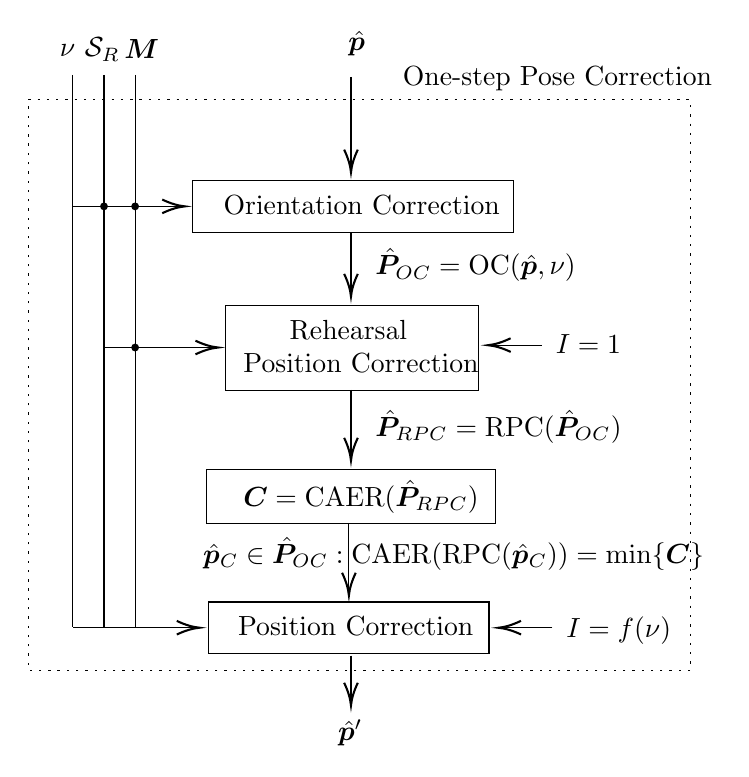
\begin{tikzpicture}[x=0.75pt,y=0.75pt,yscale=-1,xscale=1]
%uncomment if require: \path (0,542); %set diagram left start at 0, and has height of 542

%Straight Lines [id:da5372026622110897]
\draw    (126.5,63) -- (126.5,329.29) ;
%Straight Lines [id:da7972290663823844]
\draw    (260.5,64) -- (260.5,108) ;
\draw [shift={(260.5,110)}, rotate = 270] [color={rgb, 255:red, 0; green, 0; blue, 0 }  ][line width=0.75]    (10.93,-3.29) .. controls (6.95,-1.4) and (3.31,-0.3) .. (0,0) .. controls (3.31,0.3) and (6.95,1.4) .. (10.93,3.29)   ;
%Straight Lines [id:da2357744220142839]
\draw    (260.5,138.86) -- (260.5,167.86) ;
\draw [shift={(260.5,169.86)}, rotate = 270] [color={rgb, 255:red, 0; green, 0; blue, 0 }  ][line width=0.75]    (10.93,-3.29) .. controls (6.95,-1.4) and (3.31,-0.3) .. (0,0) .. controls (3.31,0.3) and (6.95,1.4) .. (10.93,3.29)   ;
%Straight Lines [id:da9232696254114303]
\draw    (352.5,193.29) -- (328.5,193.29) ;
\draw [shift={(326.5,193.29)}, rotate = 359.69] [color={rgb, 255:red, 0; green, 0; blue, 0 }  ][line width=0.75]    (10.93,-3.29) .. controls (6.95,-1.4) and (3.31,-0.3) .. (0,0) .. controls (3.31,0.3) and (6.95,1.4) .. (10.93,3.29)   ;
%Straight Lines [id:da7890748320756154]
\draw    (259.5,278.86) -- (259.5,311.86) ;
\draw [shift={(259.5,313.86)}, rotate = 270] [color={rgb, 255:red, 0; green, 0; blue, 0 }  ][line width=0.75]    (10.93,-3.29) .. controls (6.95,-1.4) and (3.31,-0.3) .. (0,0) .. controls (3.31,0.3) and (6.95,1.4) .. (10.93,3.29)   ;
%Straight Lines [id:da3579629949332166]
\draw    (260.5,342.86) -- (260.5,364.86) ;
\draw [shift={(260.5,366.86)}, rotate = 270] [color={rgb, 255:red, 0; green, 0; blue, 0 }  ][line width=0.75]    (10.93,-3.29) .. controls (6.95,-1.4) and (3.31,-0.3) .. (0,0) .. controls (3.31,0.3) and (6.95,1.4) .. (10.93,3.29)   ;
%Straight Lines [id:da8737381615370248]
\draw    (141.5,63) -- (141.5,329.29) ;
%Straight Lines [id:da6971384120103545]
\draw    (156.5,63) -- (156.5,329.29) ;
%Straight Lines [id:da8422749343405824]
\draw    (178.5,126.4) -- (156.5,126.4) ;
\draw [shift={(156.5,126.4)}, rotate = 180] [color={rgb, 255:red, 0; green, 0; blue, 0 }  ][fill={rgb, 255:red, 0; green, 0; blue, 0 }  ][line width=0.75]      (0, 0) circle [x radius= 1.35, y radius= 1.35]   ;
\draw [shift={(180.5,126.4)}, rotate = 180] [color={rgb, 255:red, 0; green, 0; blue, 0 }  ][line width=0.75]    (10.93,-3.29) .. controls (6.95,-1.4) and (3.31,-0.3) .. (0,0) .. controls (3.31,0.3) and (6.95,1.4) .. (10.93,3.29)   ;
%Straight Lines [id:da4007753539436163]
\draw    (156.5,126.4) -- (141.5,126.4) ;
\draw [shift={(141.5,126.4)}, rotate = 180] [color={rgb, 255:red, 0; green, 0; blue, 0 }  ][fill={rgb, 255:red, 0; green, 0; blue, 0 }  ][line width=0.75]      (0, 0) circle [x radius= 1.35, y radius= 1.35]   ;
%Straight Lines [id:da579363628601445]
\draw    (141.5,126.4) -- (126.5,126.4) ;
%Straight Lines [id:da5833842782446357]
\draw    (357.5,329.43) -- (333.5,329.43) ;
\draw [shift={(331.5,329.43)}, rotate = 359.69] [color={rgb, 255:red, 0; green, 0; blue, 0 }  ][line width=0.75]    (10.93,-3.29) .. controls (6.95,-1.4) and (3.31,-0.3) .. (0,0) .. controls (3.31,0.3) and (6.95,1.4) .. (10.93,3.29)   ;
%Straight Lines [id:da7806442385955334]
\draw    (260.5,214.86) -- (260.5,246.86) ;
\draw [shift={(260.5,248.86)}, rotate = 270] [color={rgb, 255:red, 0; green, 0; blue, 0 }  ][line width=0.75]    (10.93,-3.29) .. controls (6.95,-1.4) and (3.31,-0.3) .. (0,0) .. controls (3.31,0.3) and (6.95,1.4) .. (10.93,3.29)   ;
%Straight Lines [id:da6458571735202372]
\draw    (194.5,194.4) -- (156.5,194.4) ;
\draw [shift={(156.5,194.4)}, rotate = 180] [color={rgb, 255:red, 0; green, 0; blue, 0 }  ][fill={rgb, 255:red, 0; green, 0; blue, 0 }  ][line width=0.75]      (0, 0) circle [x radius= 1.35, y radius= 1.35]   ;
\draw [shift={(196.5,194.4)}, rotate = 180] [color={rgb, 255:red, 0; green, 0; blue, 0 }  ][line width=0.75]    (10.93,-3.29) .. controls (6.95,-1.4) and (3.31,-0.3) .. (0,0) .. controls (3.31,0.3) and (6.95,1.4) .. (10.93,3.29)   ;
%Straight Lines [id:da3539392704501798]
\draw    (156.5,194.5) -- (141.5,194.5) ;
%Straight Lines [id:da41656320353747733]
\draw    (185.5,329.4) -- (126.5,329.4) ;
\draw [shift={(187.5,329.4)}, rotate = 180] [color={rgb, 255:red, 0; green, 0; blue, 0 }  ][line width=0.75]    (10.93,-3.29) .. controls (6.95,-1.4) and (3.31,-0.3) .. (0,0) .. controls (3.31,0.3) and (6.95,1.4) .. (10.93,3.29)   ;
%Shape: Rectangle [id:dp8185193791005427]
\draw  [dash pattern={on 0.84pt off 2.51pt}] (105,75) -- (424,75) -- (424,350) -- (105,350) -- cycle ;
\draw (360,65) node  {One-step Pose Correction};

% Text Node
\draw    (184,114) -- (339,114) -- (339,139) -- (184,139) -- cycle  ;
\draw (189,120) node [anchor=north west][inner sep=0.75pt]   [align=left] {\ \ Orientation Correction};
% Text Node
\draw (119,47) node [anchor=north west][inner sep=0.75pt]   [align=left] {$\nu$};
% Text Node
\draw (131,44) node [anchor=north west][inner sep=0.75pt]   [align=left] {$\mathcal{S}_{R}$};
% Text Node
\draw (258,40.57) node [anchor=north west][inner sep=0.75pt]   [align=left] {$\hat{\bm{p}}$};
% Text Node
\draw (150,44.57) node [anchor=north west][inner sep=0.75pt]   [align=left] {$\bm{M}$};
% Text Node
\draw  [color={rgb, 255:red, 0; green, 0; blue, 0 }  ,draw opacity=1 ]  (200,174) -- (322,174) -- (322,215) -- (200,215) -- cycle  ;
\draw (203,180) node [anchor=north west][inner sep=0.75pt]  [align=left] {\ \ \ \ \ \ Rehearsal \\ \ Position Correction};
% Text Node
\draw    (191,253) -- (330,253) -- (330,279) -- (191,279) -- cycle  ;
\draw (194,257) node [anchor=north west][inner sep=0.75pt]   [align=left] {\ \ \ $\bm{C} = \text{CAER}(\hat{\bm{P}}_{RPC})$};
% Text Node
\draw (358,187) node [anchor=north west][inner sep=0.75pt]   [align=left] {$I = 1$};
% Text Node
\draw    (192,317) -- (327,317) -- (327,342) -- (192,342) -- cycle  ;
\draw (196,323) node [anchor=north west][inner sep=0.75pt]   [align=left] {\ \ Position Correction};
% Text Node
\draw (253,372.67) node [anchor=north west][inner sep=0.75pt]   [align=left] {$\hat{\bm{p}}^{\prime }$};
% Text Node
\draw (271,145.5) node [anchor=north west][inner sep=0.75pt]   [align=left] {$\hat{\bm{P}}_{OC} = \text{OC}(\hat{\bm{p}}, \nu)$};
% Text Node
\draw (363,323) node [anchor=north west][inner sep=0.75pt]   [align=left] {$I = f( \nu )$};
% Text Node
\draw (271,223.5) node [anchor=north west][inner sep=0.75pt]   [align=left] {$\hat{\bm{P}}_{RPC} = \text{RPC}(\hat{\bm{P}}_{OC})$};
% Text Node
\draw (188,284.5) node [anchor=north west][inner sep=0.75pt]   [align=left] {$\hat{\bm{p}}_{C} \in \hat{\bm{P}}_{OC} : \text{CAER}(\text{RPC}(\hat{\bm{p}}_C)) = \min\{\bm{C}\}$};


\end{tikzpicture}


  \caption{\small FSM iteratively invokes the One-step Pose Estimation method.
           Given a pose estimate of where scan $\mathcal{S}_1$ was captured
           within $\bm{M}$, the method attempts to register $\mathcal{S}_1$ to
           $\bm{M}$ by estimating first its relative orientation and then its
           location with respect to the input pose estimate}
  \label{fig:fsm_inner}
\end{figure}


Given an input pose estimate $\hat{\bm{p}}_1(\hat{x}_1, \hat{y}_1,
\hat{\theta}_1)$, range scan $\mathcal{S}_1$, the map $\bm{M}$, and a sampling
degree $\nu$, the One-step Pose Estimation system (fig. \ref{fig:fsm_inner})
first calculates $2^\nu$ pose estimates of $\bm{p}_1$: $\bm{P}_{OC} =
\{(\hat{x}_1, \hat{y}_1, \hat{\theta}_1^k)\}$, $k = 0,\dots,2^\nu$$-$$1$,
according to the orientation estimation method described in section
\ref{subsec:method_orientation_correction}. The initial pose estimate of
$\bm{p}_1$ is $\hat{\bm{p}}_1 = \bm{s}$.
If scans $\mathcal{S}_0$ and $\mathcal{S}_1$ were captured from the same
location, then the Percent Discrimination metric (eq. (\ref{eq:pd})) would
suffice in serving as an accurate determinant of the orientation of $\bm{p}_1$.
In practice, however, the ranking provided by the Percent Discrimination metric
is confounded by the incoincidence of the two locations. In order to mitigate
this effect, each pose estimate in $\bm{P}_{OC}$ is given over to the Position
Estimation system, where the position of each pose estimate is displaced once
($I=1$), according to the method described in section
\ref{subsec:method_location_correction}.  This operation produces the pose set
$\bm{P}_{RPC} = \{(\hat{x}_1^k, \hat{y}_1^k, \hat{\theta}_1^k)\}$,
$|\bm{P}_{RPC}| = 2^\nu$. The purpose of this operation is for it to provide an
advance view of the next step of location estimation: the less rotationally
misaligned a pose estimate of $\bm{p}_1$ is, the less it will diverge in terms
of orientation and hence position with respect to $\bm{p}_1$ once inputted to
the position estimation system (remark \ref{remark:loc_prop_or}). This
divergence is captured by the Cumulative Absolute Error per Ray (CAER) metric:
\begin{align}
  \text{CAER}_k = & \sum\limits_{n=0}^{N_s-1} \Bigg| \mathcal{S}_1[n] - \mathcal{S}_V^k[n]\Big|_{(\hat{x}_1^k, \hat{y}_1^k, \hat{\theta}_1^k)} \Bigg|
  \label{eq:caer}
\end{align}
where $\mathcal{S}_V^k$ is the map-scan captured from
$(\hat{x}_1^k, \hat{y}_1^k, \hat{\theta}_1^k)$, $k$ = $0,\dots,2^\nu$$-$$1$,
within $\bm{M}$. The CAER metric (fig. \ref{fig:caer})
encodes at the same time a degree of alignment of position and orientation
between its two input scans. By rehearsing the position estimation of each pose
estimate in $\bm{P}_{OC}$ and capturing the CAER for each of its displaced pose
estimates in $\bm{P}_{RPC}$, it is possible to establish a pose error rank
between pose estimates in $\bm{P}_{OC}$ and simultaneously retain only one pose
estimate for the next iteration of the One-step Pose Estimation
method.\footnote{Alternatively, correcting the position of $2^\nu$ pose
estimates and feeding them back to the One-step Pose Estimation method would
incur exponential costs in time of execution.} The pose estimate $\bm{p}_C \in
\bm{P}_{OC}$ which, when translated once, records the minimum CAER among all
similarly-treated pose estimates in $\bm{P}_{OC}$ is inputted to the Position
Estimation method proper. The number of translation iterations $I$ it undergoes
is an increasing function in the degree of map sampling $\nu$.
%\footnote{The rationale of chaining the number of translational
%iterations to the map sampling degree $\nu$ is the following.  Since the
%orientation error is inversely proportional to $\nu$, at low map sampling
%rates, when the position estimate error is at its highest, if the number of
%translational iterations was high then the position estimate would be
%susceptible to divergence. Therefore the number of translational iterations is
%kept low at initial stages so that a balance between decreasing position error
%and position divergence is struck. At higher values of $\nu$, the orientation
%estimate error decreases, and then divergence is bounded and/or met at higher
%translational iteration values.  As the orientation estimate becomes ever more
%accurate, the Position Estimation system is let to iterate more times so that
%further reduction of the position error be feasible.}
The Position Estimation system produces $\hat{\bm{p}}_1^\prime$, which is then
fed back to the Orientation Estimation system in the form of a new pose
estimate of $\bm{p}_1$: $\hat{\bm{p}}_1 \leftarrow \hat{\bm{p}}_1^\prime$. In
practice, the pose set $\bm{P}_{OC}$ is supplemented with one pose whose
location component is equal to $\hat{\bm{p}}_1$ and whose orientation is equal
to the orientation of $\bm{p}_C$ that produces the minimum CAER over time. This
addition introduces a form of memory to the system, which assists it in
avoiding divergence and which, therefore, benefits speed of execution.

\begin{figure}[]\hspace{1cm}
  % GNUPLOT: LaTeX picture with Postscript
\begingroup
  \makeatletter
  \providecommand\color[2][]{%
    \GenericError{(gnuplot) \space\space\space\@spaces}{%
      Package color not loaded in conjunction with
      terminal option `colourtext'%
    }{See the gnuplot documentation for explanation.%
    }{Either use 'blacktext' in gnuplot or load the package
      color.sty in LaTeX.}%
    \renewcommand\color[2][]{}%
  }%
  \providecommand\includegraphics[2][]{%
    \GenericError{(gnuplot) \space\space\space\@spaces}{%
      Package graphicx or graphics not loaded%
    }{See the gnuplot documentation for explanation.%
    }{The gnuplot epslatex terminal needs graphicx.sty or graphics.sty.}%
    \renewcommand\includegraphics[2][]{}%
  }%
  \providecommand\rotatebox[2]{#2}%
  \@ifundefined{ifGPcolor}{%
    \newif\ifGPcolor
    \GPcolorfalse
  }{}%
  \@ifundefined{ifGPblacktext}{%
    \newif\ifGPblacktext
    \GPblacktexttrue
  }{}%
  % define a \g@addto@macro without @ in the name:
  \let\gplgaddtomacro\g@addto@macro
  % define empty templates for all commands taking text:
  \gdef\gplbacktext{}%
  \gdef\gplfronttext{}%
  \makeatother
  \ifGPblacktext
    % no textcolor at all
    \def\colorrgb#1{}%
    \def\colorgray#1{}%
  \else
    % gray or color?
    \ifGPcolor
      \def\colorrgb#1{\color[rgb]{#1}}%
      \def\colorgray#1{\color[gray]{#1}}%
      \expandafter\def\csname LTw\endcsname{\color{white}}%
      \expandafter\def\csname LTb\endcsname{\color{black}}%
      \expandafter\def\csname LTa\endcsname{\color{black}}%
      \expandafter\def\csname LT0\endcsname{\color[rgb]{1,0,0}}%
      \expandafter\def\csname LT1\endcsname{\color[rgb]{0,1,0}}%
      \expandafter\def\csname LT2\endcsname{\color[rgb]{0,0,1}}%
      \expandafter\def\csname LT3\endcsname{\color[rgb]{1,0,1}}%
      \expandafter\def\csname LT4\endcsname{\color[rgb]{0,1,1}}%
      \expandafter\def\csname LT5\endcsname{\color[rgb]{1,1,0}}%
      \expandafter\def\csname LT6\endcsname{\color[rgb]{0,0,0}}%
      \expandafter\def\csname LT7\endcsname{\color[rgb]{1,0.3,0}}%
      \expandafter\def\csname LT8\endcsname{\color[rgb]{0.5,0.5,0.5}}%
    \else
      % gray
      \def\colorrgb#1{\color{black}}%
      \def\colorgray#1{\color[gray]{#1}}%
      \expandafter\def\csname LTw\endcsname{\color{white}}%
      \expandafter\def\csname LTb\endcsname{\color{black}}%
      \expandafter\def\csname LTa\endcsname{\color{black}}%
      \expandafter\def\csname LT0\endcsname{\color{black}}%
      \expandafter\def\csname LT1\endcsname{\color{black}}%
      \expandafter\def\csname LT2\endcsname{\color{black}}%
      \expandafter\def\csname LT3\endcsname{\color{black}}%
      \expandafter\def\csname LT4\endcsname{\color{black}}%
      \expandafter\def\csname LT5\endcsname{\color{black}}%
      \expandafter\def\csname LT6\endcsname{\color{black}}%
      \expandafter\def\csname LT7\endcsname{\color{black}}%
      \expandafter\def\csname LT8\endcsname{\color{black}}%
    \fi
  \fi
    \setlength{\unitlength}{0.0500bp}%
    \ifx\gptboxheight\undefined%
      \newlength{\gptboxheight}%
      \newlength{\gptboxwidth}%
      \newsavebox{\gptboxtext}%
    \fi%
    \setlength{\fboxrule}{0.5pt}%
    \setlength{\fboxsep}{1pt}%
\begin{picture}(4000.00,2000.00)%
    \gplgaddtomacro\gplbacktext{%
    }%
    \gplgaddtomacro\gplfronttext{%
      \colorrgb{0.15,0.15,0.15}%
      \put(326,220){\makebox(0,0)[r]{\strut{}$0.0$}}%
      \colorrgb{0.15,0.15,0.15}%
      \put(326,446){\makebox(0,0)[r]{\strut{}$0.05$}}%
      \colorrgb{0.15,0.15,0.15}%
      \put(326,672){\makebox(0,0)[r]{\strut{}$0.10$}}%
      \colorrgb{0.15,0.15,0.15}%
      \put(326,897){\makebox(0,0)[r]{\strut{}$0.15$}}%
      \colorrgb{0.15,0.15,0.15}%
      \put(326,1122){\makebox(0,0)[r]{\strut{}$0.20$}}%
      \colorrgb{0.15,0.15,0.15}%
      \put(326,1348){\makebox(0,0)[r]{\strut{}$0.25$}}%
      \colorrgb{0.15,0.15,0.15}%
      \put(326,1574){\makebox(0,0)[r]{\strut{}$0.30$}}%
      \colorrgb{0.15,0.15,0.15}%
      \put(326,1799){\makebox(0,0)[r]{\strut{}$0.35$}}%
      \colorrgb{0.15,0.15,0.15}%
      \put(-285,1010){\rotatebox{90}{\makebox(0,0){\strut{}$(\Delta x^2 + \Delta y^2)^{1/2}$ [m]}}}%
      \colorrgb{0.15,0.15,0.15}%
      \put(533,80){\makebox(0,0){\strut{}$-\frac{{\pi}}{4}$}}%
      \colorrgb{0.15,0.15,0.15}%
      \put(1150,80){\makebox(0,0){\strut{}$-\frac{{\pi}}{8}$}}%
      \colorrgb{0.15,0.15,0.15}%
      \put(1459,80){\makebox(0,0){\strut{}$-\frac{{\pi}}{16}$}}%
      \colorrgb{0.15,0.15,0.15}%
      \put(1767,80){\makebox(0,0){\strut{}$0$}}%
      \colorrgb{0.15,0.15,0.15}%
      \put(2075,80){\makebox(0,0){\strut{}$+\frac{{\pi}}{16}$}}%
      \colorrgb{0.15,0.15,0.15}%
      \put(2384,80){\makebox(0,0){\strut{}$+\frac{{\pi}}{8}$}}%
      \colorrgb{0.15,0.15,0.15}%
      \put(3001,80){\makebox(0,0){\strut{}$+\frac{{\pi}}{4}$}}%
      \colorrgb{0.15,0.15,0.15}%
      \put(1767,-275){\makebox(0,0){\strut{}$\Delta\theta$ [rad]}}%
    }%
    \gplgaddtomacro\gplbacktext{%
    }%
    \gplgaddtomacro\gplfronttext{%
      \colorrgb{0.15,0.15,0.15}%
      \put(3627,185){\makebox(0,0)[l]{\strut{}$0$}}%
      \colorrgb{0.15,0.15,0.15}%
      \put(3627,444){\makebox(0,0)[l]{\strut{}$100$}}%
      \colorrgb{0.15,0.15,0.15}%
      \put(3627,703){\makebox(0,0)[l]{\strut{}$200$}}%
      \colorrgb{0.15,0.15,0.15}%
      \put(3627,963){\makebox(0,0)[l]{\strut{}$300$}}%
      \colorrgb{0.15,0.15,0.15}%
      \put(3627,1222){\makebox(0,0)[l]{\strut{}$400$}}%
      \colorrgb{0.15,0.15,0.15}%
      \put(3627,1481){\makebox(0,0)[l]{\strut{}$500$}}%
      \colorrgb{0.15,0.15,0.15}%
      \put(3627,1741){\makebox(0,0)[l]{\strut{}$600$}}%
    }%
    \gplbacktext
    \put(0,0){
\includegraphics{./figures/caer}}%
    \gplfronttext
  \end{picture}%
\endgroup

  \vspace{1cm}
  \caption{\small A profile of the CAER metric (eq. (\ref{eq:caer})) from
           $10^6$ pairs of sample scans, depending on the distance
           $(\Delta x^2 + \Delta y^2)^{1/2}$ and relative orientation
           $\Delta \theta$ of the poses from where the two scans were captured.
           Pose estimates closer to the true pose in terms of orientation
           (a) exhibit lower CAER values than those further away from it and (b)
           produce lower location errors once inputted to the Location
           Estimation system}
  \label{fig:caer}
\end{figure}

Given pose $\hat{\bm{p}}_1$, range scan $\mathcal{S}_1$, and the map $\bm{M}$,
the pose estimation method proposed iteratively invokes the One-step Pose
Estimation process until a set of termination conditions is met. Denoting the
former by FSM (Fourier Scan Matching), FSM starts off with an initial degree of
sampling the map $\nu$ = $\nu_{\min}$. The input pose estimate
$\hat{\bm{p}}_1$ is processed by the One-step Pose Estimation process, and its
output $\hat{\bm{p}}_1^\prime$ is examined with regard to Recovery and
Convergence conditions. If the resulting pose estimate falls outside of the map
$\bm{M}$ then a new pose estimate is generated from the initially supplied pose
estimate $\bm{s}$, and the process is reset.  If no significant pose estimate
correction is observed $\|\hat{\bm{p}}_1^\prime-\hat{\bm{p}}_1\|_2 <
\varepsilon_{\delta p}$, then the degree of map sampling $\nu$ is increased.
Its increase serves as a means of reducing the orientation and hence the
position estimate error further.  Otherwise, the One-step Pose Estimation
process is iterated until a maximum degree of map sampling is reached $\nu$ =
$\nu_{\max}$, at which point FSM terminates. Its output is
$\hat{\bm{p}}_1^\prime$, which is the pose estimate of $\bm{p}_1$ in the frame
of reference of $\bm{M}$. The roto-translation
$\hat{\bm{T}} = \hat{\bm{p}}_1^\prime - \bm{s} = \hat{\bm{p}}_1^\prime$ is the
estimate of the sensor's true motion $\bm{T}$.



%%%%%%%%%%%%%%%%%%%%%%%%%%%%%%%%%%%%%%%%%%%%%%%%%%%%%%%%%%%%%%%%%%%%%%%%%%%%%%%%
\section{Results}
  \label{section:results}
  %%%%%%%%%%%%%%%%%%%%%%%%%%%%%%%%%%%%%%%%%%%%%%%%%%%%%%%%%%%%%%%%%%%%%%%%%%%%%%%%
\subsection{Experimental Design}
  \label{section:experimental}
  The experimental procedure was conducted using a benchmark dataset $D$
consisting of $|D| = 778$ laser scans obtained from a Sick range-scan sensor
mounted on a robotic wheel-chair \cite{dataset_link}. For
each scan $D^d$, $d = 1,\dots,778$, the dataset reports one range scan of $360$
range measurements and the pose from which it was captured
$\bm{r}^d(x,y,\theta)$.  The same dataset was used to evaluate the performance
of IDC \cite{LuMilios}, ICP, and MBICP in \cite{mbicp}, and that of PLICP and
the joint method PLICP$\circ$GPM during scan-matching experiments. In
\cite{plicp} the latter was found to be the best-performing among the five
correspondence-finding scan-matching methods. Therefore, for purposes of
comparison against correspondence-finding scan-matching methods, the
experimental procedure is extended to PLICP$\circ$GPM. This method shall be
denoted hereafter by the acronym CSM. In the same vein, for purposes of
comparison against correspondenceless scan-matching methods, the same
experimental procedure is extended to the Normal Distributions Transform (NDT)
scan-matching method \cite{ndt1}.

The experimental setup is the following. The rays of each dataset instance
$D^d$ are first projected to the $x-y$ plane around $\bm{r}^d$. The dataset's
scans are not panoramic, therefore the remaining space is filled with a
semicircular arc that joins the scan's two extreme ends. Similar fashions for
closing-off the environment have been found equivalent with respect to the
performance of the tested methods. The resulting point-set is regarded as the
environment $\bm{W}^d$ in which the range sensor operates.  Then the pose
$\bm{p}_0^d$ from which $\mathcal{S}_0^d$ is captured is generated randomly
within the polygon formed by $\bm{W}^d$. The pose $\bm{p}_1^d$ from which the
sensor captured $\mathcal{S}_1$ is then obtained by perturbing the components
of $\bm{p}_0^d$ with quantities extracted from uniformly distributed error
distributions $U_{xy}(-\overline{\delta}_{xy}, \overline{\delta}_{xy})$,
$U_{\theta}(-\overline{\delta}_{\theta}, \overline{\delta}_{\theta})$;
$\overline{\delta}_{xy}$, $\overline{\delta}_\theta$ $\in \mathbb{R}_{\geq 0}$.
?? TODO say that censi et al did not test this but tested self-scan-matching ??


Range scans $\mathcal{S}_0^d$ and $\mathcal{S}_1^d$ are then computed by
locating the intersection points between $N_s$ rays emanating from $\bm{p}_0^d$
and $\bm{p}_1^d$, respectively, and the polygon formed by $\bm{W}^d$ across an
angular field of view $\lambda = 2\pi$. The inputs to CSM, NDT, and FSM are
then set to $\mathcal{S}_0^d$ and $\mathcal{S}_1^d$. Their output is
$\bm{p}_1^{\prime d}$. The roto-translation
$\hat{\bm{T}}^d = \bm{p}_1^{\prime d}$ is the estimate of the motion
$\bm{T}^d = \bm{p}_1^d - \bm{p}_0^d$ of the range sensor. The criterion on
which the evaluation of all experiments rests is the $2$-norm of the total pose
displacement error
\begin{align}
  e^d &= \| \bm{T}^d - \hat{\bm{T}}^d \|_2
  \label{eq:rototranslation_error}
\end{align}

For every pose estimate $\bm{p}_1^{\prime d}$ outputted by
each algorithm, $d = 1,2,\dots,|D|$, its offset from the actual pose
$\bm{p}_1^d$ is recorded in the form of the $2$-norm total error. The pose
errors of one experiment are then averaged. The pose error distributions
reported below are those of mean errors across $E$ experiments of the same
configuration.

In order to test for the performance of the proposed method with use of real
sensors, five levels of noise acting on the range measurements of the scans are
tested. The range measurements are perturbed by zero-mean normally-distributed
noise with standard deviation $\sigma_R \in \{0.0, 0.01, 0.03, 0.05, 0.10\}$ m.
The non-zero values of tested standard deviations were calculated from
commercially available panoramic LIDAR scanners by identifying the magnitude of
their reported maximum range errors and dividing it by a factor of three. The
rationale is that $99.73\%$ of errors are located within $3\sigma$ around the
actual range between a ray and an obstacle, assuming errors are distributed
normally. The minimum standard deviation $\sigma_R = 0.01$ m is reported for
VELODYNE sensors \cite{velodyne_datasheet}; the rest are reported for
price-appealing but disturbance-laden sensors, e.g. the RPLIDAR A2M8, or the
YDLIDAR G4, TG30, and X4 scanners \cite{a2m8_datasheet}-\cite{x4_datasheet}. The
size of the input scans was set to $N_s=360$ rays. The minimum and maximum map
oversampling rates of FSM were set to $(\mu_{\min},\mu_{\max}) =
(2^{\nu_{\min}},2^{\nu_{\max}}) = (2^0,2^3)$. The number of iterations of the
translational component at each map sampling degree $\nu$ was set at $I =
2\nu$. The orientation convergence threshold was set to $\varepsilon_{\delta p}
= 10$e-$5$. Maximal displacements $\overline{\delta}_{xy}$ and
$\overline{\delta}_\theta$ were chosen as such by prior art tests \cite{plicp}.
For each experiment FSM, CSM, and NDT ran for $E = 100$ times across all
instances of $D$. Therefore each method underwent a total of
$100 \times 778 \times 6 \times 5 \sim O(10^6)$ experiments.
All experiments and algorithms were run serially, in C++, on
a single thread, on a machine with a CPU frequency of $4.0$ GHz. The
implementations of CSM and NDT were taken from \cite{csm_implementation} and
\cite{ndt_implementation} respectively.


%%%%%%%%%%%%%%%%%%%%%%%%%%%%%%%%%%%%%%%%%%%%%%%%%%%%%%%%%%%%%%%%%%%%%%%%%%%%%%%%
\subsection{Performance}
  \label{section:performance}
  Figure \ref{fig:errors_sm} shows the distribution of roto-translation errors
(eq. (\ref{eq:rototranslation_error})) across $E$ experiments for CSM (red),
NDT (blue), and the proposed method of FSM (green).

\begin{figure}[]\centering
  % GNUPLOT: LaTeX picture with Postscript
\begingroup
  \makeatletter
  \providecommand\color[2][]{%
    \GenericError{(gnuplot) \space\space\space\@spaces}{%
      Package color not loaded in conjunction with
      terminal option `colourtext'%
    }{See the gnuplot documentation for explanation.%
    }{Either use 'blacktext' in gnuplot or load the package
      color.sty in LaTeX.}%
    \renewcommand\color[2][]{}%
  }%
  \providecommand\includegraphics[2][]{%
    \GenericError{(gnuplot) \space\space\space\@spaces}{%
      Package graphicx or graphics not loaded%
    }{See the gnuplot documentation for explanation.%
    }{The gnuplot epslatex terminal needs graphicx.sty or graphics.sty.}%
    \renewcommand\includegraphics[2][]{}%
  }%
  \providecommand\rotatebox[2]{#2}%
  \@ifundefined{ifGPcolor}{%
    \newif\ifGPcolor
    \GPcolorfalse
  }{}%
  \@ifundefined{ifGPblacktext}{%
    \newif\ifGPblacktext
    \GPblacktexttrue
  }{}%
  % define a \g@addto@macro without @ in the name:
  \let\gplgaddtomacro\g@addto@macro
  % define empty templates for all commands taking text:
  \gdef\gplfronttext{}%
  \gdef\gplfronttext{}%
  \makeatother
  \ifGPblacktext
    % no textcolor at all
    \def\colorrgb#1{}%
    \def\colorgray#1{}%
  \else
    % gray or color?
    \ifGPcolor
      \def\colorrgb#1{\color[rgb]{#1}}%
      \def\colorgray#1{\color[gray]{#1}}%
      \expandafter\def\csname LTw\endcsname{\color{white}}%
      \expandafter\def\csname LTb\endcsname{\color{black}}%
      \expandafter\def\csname LTa\endcsname{\color{black}}%
      \expandafter\def\csname LT0\endcsname{\color[rgb]{1,0,0}}%
      \expandafter\def\csname LT1\endcsname{\color[rgb]{0,1,0}}%
      \expandafter\def\csname LT2\endcsname{\color[rgb]{0,0,1}}%
      \expandafter\def\csname LT3\endcsname{\color[rgb]{1,0,1}}%
      \expandafter\def\csname LT4\endcsname{\color[rgb]{0,1,1}}%
      \expandafter\def\csname LT5\endcsname{\color[rgb]{1,1,0}}%
      \expandafter\def\csname LT6\endcsname{\color[rgb]{0,0,0}}%
      \expandafter\def\csname LT7\endcsname{\color[rgb]{1,0.3,0}}%
      \expandafter\def\csname LT8\endcsname{\color[rgb]{0.5,0.5,0.5}}%
    \else
      % gray
      \def\colorrgb#1{\color{black}}%
      \def\colorgray#1{\color[gray]{#1}}%
      \expandafter\def\csname LTw\endcsname{\color{white}}%
      \expandafter\def\csname LTb\endcsname{\color{black}}%
      \expandafter\def\csname LTa\endcsname{\color{black}}%
      \expandafter\def\csname LT0\endcsname{\color{black}}%
      \expandafter\def\csname LT1\endcsname{\color{black}}%
      \expandafter\def\csname LT2\endcsname{\color{black}}%
      \expandafter\def\csname LT3\endcsname{\color{black}}%
      \expandafter\def\csname LT4\endcsname{\color{black}}%
      \expandafter\def\csname LT5\endcsname{\color{black}}%
      \expandafter\def\csname LT6\endcsname{\color{black}}%
      \expandafter\def\csname LT7\endcsname{\color{black}}%
      \expandafter\def\csname LT8\endcsname{\color{black}}%
    \fi
  \fi
  \setlength{\unitlength}{0.0500bp}%
  \begin{picture}(5000.00,12000.00)%
    \gplgaddtomacro\gplfronttext{%
      \colorrgb{0.00,0.00,0.00}%
      \put(518,10003){\makebox(0,0)[r]{\strut{}$0.0$}}%
      \colorrgb{0.00,0.00,0.00}%
      \put(518,10186){\makebox(0,0)[r]{\strut{}$0.005$}}%
      \colorrgb{0.00,0.00,0.00}%
      \put(518,10368){\makebox(0,0)[r]{\strut{}$0.01$}}%
      \colorrgb{0.00,0.00,0.00}%
      \put(518,10551){\makebox(0,0)[r]{\strut{}$0.015$}}%
      \colorrgb{0.00,0.00,0.00}%
      \put(518,10734){\makebox(0,0)[r]{\strut{}$0.02$}}%
      \colorrgb{0.00,0.00,0.00}%
      \put(518,10916){\makebox(0,0)[r]{\strut{}$0.025$}}%
      \colorrgb{0.00,0.00,0.00}%
      \put(518,11099){\makebox(0,0)[r]{\strut{}$0.03$}}%
      \colorrgb{0.00,0.00,0.00}%
      \put(2587,11329){\makebox(0,0){\strut{}$(\overline{\delta}_{xy}, \overline{\delta}_\theta) = (0.05 \ \text{m}, 2^\circ)$}}%
      \put(2487,11729){\makebox(0,0){\strut{}Distribution of mean roto-translation errors [(m$^2$ + rad$^2$)$^{1/2}$]}}%
    }%
    \gplgaddtomacro\gplfronttext{%
    }%
    \gplgaddtomacro\gplfronttext{%
      \colorrgb{0.00,0.00,0.00}%
      \put(518,8266){\makebox(0,0)[r]{\strut{}$0.0$}}%
      \colorrgb{0.00,0.00,0.00}%
      %\put(518,8403){\makebox(0,0)[r]{\strut{}$0.005$}}%
      \colorrgb{0.00,0.00,0.00}%
      \put(518,8540){\makebox(0,0)[r]{\strut{}$0.01$}}%
      \colorrgb{0.00,0.00,0.00}%
      %\put(518,8677){\makebox(0,0)[r]{\strut{}$0.015$}}%
      \colorrgb{0.00,0.00,0.00}%
      \put(518,8814){\makebox(0,0)[r]{\strut{}$0.02$}}%
      \colorrgb{0.00,0.00,0.00}%
      %\put(518,8951){\makebox(0,0)[r]{\strut{}$0.025$}}%
      \colorrgb{0.00,0.00,0.00}%
      \put(518,9088){\makebox(0,0)[r]{\strut{}$0.03$}}%
      \colorrgb{0.00,0.00,0.00}%
      %\put(518,9225){\makebox(0,0)[r]{\strut{}$0.035$}}%
      \colorrgb{0.00,0.00,0.00}%
      \put(518,9362){\makebox(0,0)[r]{\strut{}$0.04$}}%
      \colorrgb{0.00,0.00,0.00}%
      \put(2587,9592){\makebox(0,0){\strut{}$(\overline{\delta}_{xy}, \overline{\delta}_\theta) = (0.10 \ \text{m}, 4^\circ)$}}%
    }%
    \gplgaddtomacro\gplfronttext{%
    }%
    \gplgaddtomacro\gplfronttext{%
      \colorrgb{0.00,0.00,0.00}%
      \put(518,6530){\makebox(0,0)[r]{\strut{}$0.0$}}%
      \colorrgb{0.00,0.00,0.00}%
      \put(518,6749){\makebox(0,0)[r]{\strut{}$0.01$}}%
      \colorrgb{0.00,0.00,0.00}%
      \put(518,6968){\makebox(0,0)[r]{\strut{}$0.02$}}%
      \colorrgb{0.00,0.00,0.00}%
      \put(518,7188){\makebox(0,0)[r]{\strut{}$0.03$}}%
      \colorrgb{0.00,0.00,0.00}%
      \put(518,7407){\makebox(0,0)[r]{\strut{}$0.04$}}%
      \colorrgb{0.00,0.00,0.00}%
      \put(518,7626){\makebox(0,0)[r]{\strut{}$0.05$}}%
      \colorrgb{0.00,0.00,0.00}%
      \put(2587,7856){\makebox(0,0){\strut{}$(\overline{\delta}_{xy}, \overline{\delta}_\theta) = (0.15 \ \text{m}, 8.6^\circ)$}}%
    }%
    \gplgaddtomacro\gplfronttext{%
    }%
    \gplgaddtomacro\gplfronttext{%
      \colorrgb{0.00,0.00,0.00}%
      \put(518,4793){\makebox(0,0)[r]{\strut{}$0.0$}}%
      \colorrgb{0.00,0.00,0.00}%
      \put(518,4976){\makebox(0,0)[r]{\strut{}$0.01$}}%
      \colorrgb{0.00,0.00,0.00}%
      \put(518,5158){\makebox(0,0)[r]{\strut{}$0.02$}}%
      \colorrgb{0.00,0.00,0.00}%
      \put(518,5341){\makebox(0,0)[r]{\strut{}$0.03$}}%
      \colorrgb{0.00,0.00,0.00}%
      \put(518,5524){\makebox(0,0)[r]{\strut{}$0.04$}}%
      \colorrgb{0.00,0.00,0.00}%
      \put(518,5706){\makebox(0,0)[r]{\strut{}$0.05$}}%
      \colorrgb{0.00,0.00,0.00}%
      \put(518,5889){\makebox(0,0)[r]{\strut{}$0.06$}}%
      \colorrgb{0.00,0.00,0.00}%
      \put(2587,6119){\makebox(0,0){\strut{}$(\overline{\delta}_{xy}, \overline{\delta}_\theta) = (0.20 \ \text{m}, 17.2^\circ)$}}%
    }%
    \gplgaddtomacro\gplfronttext{%
    }%
    \gplgaddtomacro\gplfronttext{%
      \colorrgb{0.00,0.00,0.00}%
      \put(518,3056){\makebox(0,0)[r]{\strut{}$0.0$}}%
      \colorrgb{0.00,0.00,0.00}%
      \put(518,3275){\makebox(0,0)[r]{\strut{}$0.02$}}%
      \colorrgb{0.00,0.00,0.00}%
      \put(518,3494){\makebox(0,0)[r]{\strut{}$0.04$}}%
      \colorrgb{0.00,0.00,0.00}%
      \put(518,3714){\makebox(0,0)[r]{\strut{}$0.06$}}%
      \colorrgb{0.00,0.00,0.00}%
      \put(518,3933){\makebox(0,0)[r]{\strut{}$0.08$}}%
      \colorrgb{0.00,0.00,0.00}%
      \put(518,4152){\makebox(0,0)[r]{\strut{}$0.10$}}%
      \colorrgb{0.00,0.00,0.00}%
      \put(2587,4382){\makebox(0,0){\strut{}$(\overline{\delta}_{xy}, \overline{\delta}_\theta) = (0.20 \ \text{m}, 32^\circ)$}}%
    }%
    \gplgaddtomacro\gplfronttext{%
    }%
    \gplgaddtomacro\gplfronttext{%
      \colorrgb{0.00,0.00,0.00}%
      \put(518,1320){\makebox(0,0)[r]{\strut{}$0.0$}}%
      \colorrgb{0.00,0.00,0.00}%
      \put(518,1594){\makebox(0,0)[r]{\strut{}$0.05$}}%
      \colorrgb{0.00,0.00,0.00}%
      \put(518,1868){\makebox(0,0)[r]{\strut{}$0.10$}}%
      \colorrgb{0.00,0.00,0.00}%
      \put(518,2142){\makebox(0,0)[r]{\strut{}$0.15$}}%
      \colorrgb{0.00,0.00,0.00}%
      \put(518,2416){\makebox(0,0)[r]{\strut{}$0.20$}}%
      \colorrgb{0.00,0.00,0.00}%
      \put(1037,1100){\makebox(0,0){\strut{}$0.0$}}%
      \colorrgb{0.00,0.00,0.00}%
      \put(1812,1100){\makebox(0,0){\strut{}$0.01$}}%
      \colorrgb{0.00,0.00,0.00}%
      \put(2587,1100){\makebox(0,0){\strut{}$0.03$}}%
      \colorrgb{0.00,0.00,0.00}%
      \put(3362,1100){\makebox(0,0){\strut{}$0.05$}}%
      \colorrgb{0.00,0.00,0.00}%
      \put(4137,1100){\makebox(0,0){\strut{}$0.10$}}%
      \colorrgb{0.00,0.00,0.00}%
      \put(2587,770){\makebox(0,0){\strut{}sd of sensor measurement noise $\sigma_R$ [m]}}%
      \colorrgb{0.00,0.00,0.00}%
      \put(2587,2646){\makebox(0,0){\strut{}$(\overline{\delta}_{xy}, \overline{\delta}_\theta) = (0.20 \ \text{m}, 45^\circ)$}}%
    }%
    \put(0,0){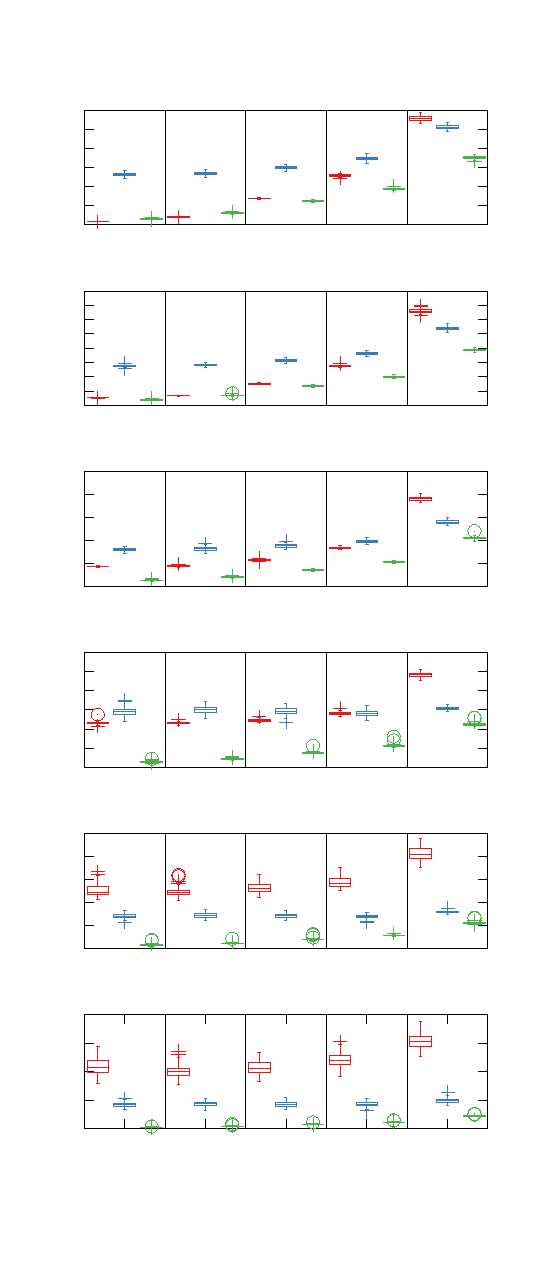
\includegraphics{./figures/experiments/errors_CSM_NDT_implm6_short}}%
    \gplfronttext
  \end{picture}%
\endgroup

  \caption{\small Distribution of mean errors of CSM (red), NDT (blue), and
           FSM (our approach) across a range of maximal positional and
           orientational displacements, for progressively larger sensor
           measurement noise levels. The variability of FSM's rigid body
           transformation error is consistent across all configurations. The
           error is independent of the initial displacement of scans for a
           given level of sensor noise}
  \label{fig:errors_sm}
\end{figure}

At small location and orientation displacements between the two input scans
($\overline{\delta}_{xy} \leq $ 0.05 m,
$\overline{\delta}_\theta \leq 2^\circ$), CSM outperforms NDT and FSM for low
levels of sensor noise ($\sigma_R \leq 0.01$ m). However, as noise increases,
FSM starts exhibiting greater robustness and accuracy than CSM. At
greater location and orientation displacements
($\overline{\delta}_{xy} > 0.05$ m,
$\overline{\delta}_\theta > 2^\circ$), FSM is able to maintain errors equal to
or lower than CSM across the entirety of the spectrum of tested noise levels.
Compared to the equally correspondenceless method of NDT, FSM exhibits greater
accuracy across all tested configurations. The variability of FSM's errors
for a given level of sensor noise is independent of the displacement of the
two input scans. The juxtaposition of the three methods' pose errors at high
levels of sensor noise highlight the robustness afforded to FSM by the Discrete
Fourier transform and its properties. In terms of execution time, CSM ranged
from $4.8$ to $20.5$ ms, NDT from $8.1$ to $19.9$ ms, and FSM from $13.2$ to
$16.7$ ms. Therefore FSM's exhibits the least variability to sensor noise and
locational and orientational displacement in terms of runtime. The measurement
frequency of modern LIDAR sensors ranges from $12$-$20$ Hz; therefore FSM runs
in real time in modern processors.



%%%%%%%%%%%%%%%%%%%%%%%%%%%%%%%%%%%%%%%%%%%%%%%%%%%%%%%%%%%%%%%%%%%%%%%%%%%%%%%%
\section{Conclusions}
  \label{section:finale}
  This paper has presented a real-time scan-matching method for panoramic 2D LIDAR
sensors. The approach rests on properties of the DFT, which afford it
increased robustness and accuracy compared to state-of-the-art scan-matching
approaches in the face of measurement noise exhibited by real-life sensors.
FSM does not rely on correspondences or features, and may operate under missing
range information; it is suitable for unstructured and outdoor environments,
even with high-frequency components.

Future work will focus on extending FSM to 3D LIDAR sensors, either by extension
to the slices not parallel to the ground, which may provide vertical motion
information according to the sine of each slice's pitch angle, or by
generalising its two main submethods to the 3D/6DOF space.

The C++ code of the proposed method, along with the implementation of the
conducted experiments is available at \url{https://github.com/li9i/fsm}.


%%%%%%%%%%%%%%%%%%%%%%%%%%%%%%%%%%%%%%%%%%%%%%%%%%%%%%%%%%%%%%%%%%%%%%%%%%%%%%%%
\newpage
\begin{thebibliography}{99}
  \input{./sections/bibliography.bib}
\end{thebibliography}

%%%%%%%%%%%%%%%%%%%%%%%%%%%%%%%%%%%%%%%%%%%%%%%%%%%%%%%%%%%%%%%%%%%%%%%%%%%%%%%%
% This command serves to balance the column lengths
% on the last page of the document manually. It shortens
% the textheight of the last page by a suitable amount.
% This command does not take effect until the next page
% so it should come on the page before the last. Make
% sure that you do not shorten the textheight too much.
%\addtolength{\textheight}{-1cm}

\balance

\end{document}
